\documentclass[12pt]{ruthesis}
\usepackage{amsmath}
\usepackage{amssymb}
\usepackage{latexsym}
\usepackage{graphics}
\usepackage{epsfig,epsf,rotating}
\usepackage{subfigure}
\usepackage{color}
\usepackage{epsf}
\usepackage{algorithm} % for the algorithm environment
\usepackage{algpseudocode}
\usepackage{theorem}
\newtheorem{proposition}{Proposition}

\theoremheaderfont{\itshape} {\theoremstyle{break}
\newtheorem{Fact}{Fact}[chapter]} \theoremstyle{break}
\newtheorem{Lem}{Lemma}[chapter] \theoremstyle{break}
\newtheorem{Thm}{Theorem}[chapter] {\theoremstyle{plain}
  \theorembodyfont{\rmfamily}  \newtheorem{Prf}{Proof}[chapter]}
{\theoremstyle{plain}
  \theorembodyfont{\rmfamily}  \newtheorem{Def}{Definition}[chapter]}

% new commands.
\algnewcommand{\LineComment}[1]{\State\(\triangleright\) #1}
% Comments for the whole line

\title{Low cost \emph{ab initio} methods for weak and strong electronic 
correlation}

\author{Roman Schutsky}
\department{Chemistry}
\school{Rice University}
\degree{Doctor of Philosophy}

\committee {
        Gustavo E. Scuseria, Chair \\
        Professor of Chemistry and Physics and Astronomy \and
        Anatoly Kolomeiski \\
        Professor of Chemistry\and
        Boris Yakobson\\
        Professor of Materials Science and NanoEngineering and Chemistry
}

\address{Houston, Texas}
\donemonth{Jan} \doneyear{2018} \makeindex
\begin{document}

  \begin{frontmatter}
   \pagenumbering{roman}
   %\makecover
   \maketitle
   \thispagestyle{empty}
\begin{abstract}
Ever increasing demand for high data rate wireless transmissions with high spectral efficiency leads to utilization of communication systems with multiple transmit and receive antennas. In addition, excellent error-rate performance can be achieved with iterative receiver structure composed of inner detection and outer decoding. In this work we design algorithms and architectures for iterative wireless receivers with multiple antennas that are applied in both downlink and uplink scenarios. It is our goal to develop wireless receivers with implementable hardware cost, excellent error-rate performance while achieving high data rates in the order of 1 Gbps.

Soft sphere detection algorithm with reduced computational complexity based on probabilistically bounded candidate-search process is proposed. The error-rate performance are improved compare to other bounded soft sphere detection schemes for the same hardware cost. Partial candidate-search process called QRD-QLD detection is also developed for fast mobile downlink receivers. It has significantly smaller detection latency than the well-known QRD-M algorithm proposed for several emerging wireless systems. The error-rate performance are equivalent for identical hardware complexity. We apply bounded soft sphere detection in the single-carrier uplink receiver specified for the 3GPP-LTE wireless standard. By applying sphere post-detection after MMSE-based channel pre-equalization, the interference from multiple users is successfully suppressed with limited increase of computational complexity. Cost-efficient high-speed architecture design of soft sphere detector based on bounded candidate-search has been also implemented. 

Outer LDPC decoding is used at the receiver back-end. Different levels of processing parallelism for outer structured semi-parallel LDPC decoders are investigated. We propose estimation methodology that quickly and accurately determines decoder architecture with the best tradeoff between area cost, decoding throughput and error-rate performance. Two decoder architectures with different levels of processing parallelism are implemented. Block-structured LDPC codes are designed for particular inner soft sphere detector and channel environment supporting modular high-speed decoder architectures. Finally, we propose methodology to estimate level of processing parallelism for the physical layer portion of iterative receiver necessary to achieve real-time data-rates of future wireless systems, such as the 1 Gbps downlink transmission.
\end{abstract}



   %\include{ack}
   \tableofcontents
   \listoffigures
   \listoftables
%   \include{ded}
  \end{frontmatter}
\pagenumbering{arabic}

\linespacing{1.7}

\chapter{Introduction}
\label{ch:Intro}
Ever increasing demand for high data rate wireless transmissions with high spectral efficiency leads to utilization of communication systems with multiple transmit and receive antennas. Excellent quality of service represented with near-channel capacity error-rate performance can be achieved with iterative receiver structure composed of inner soft detection and outer soft-input soft-output decoding. Emerging wireless standards such as:~Wireless Local Area Network (W-LAN), Worldwide Interoperability for Microwave Access (WiMAX), $3^{rd}$ Generation Partnership Project Long Term Evolution (3GPP-LTE), etc are being constantly revised to provide higher data rates and better error-rate performance. Iterative receivers based on inner soft detection and outer decoding are promising solutions.

In this thesis, we propose to address issues of designing efficient physical layer receiver structure targeting its use in emerging wireless systems, including both downlink and uplink scenarios. It is our goal to develop performance-efficient wireless receiver with implementable hardware cost while achieving data throughputs in the order of hundreds MBits/sec. 

\section{Motivation}
\label{sec:Motivation}
Excellent error-rate performance in MIMO environment are made possible by employing sophisticated algorithms such as maximum \emph{a posteriori}~(MAP) detection techniques and outer channel decoding that provides error-correction in the presence of multiple access interference, burst channel fading, channel multi-paths, additive receiver noise, etc. An approximation of impractically complex optimal joint detection/decoding is achieved by iteratively improving the \emph{a posteriori} probabilities (APPs) of transmitted coded bits between inner soft detection and outer decoding~\cite{HochwaldTC03}. Inner detection is typically based on the simplification of exponentially complex maximum-likelihood~(ML) approach such as the sphere detection~\cite{FinckeMC85}. 
\chapter{Tensor structured Coupled Cluster}
\label{ch:tcc} 
The discussion presented in this section based on our published work, see 
Ref.~\cite{schutski2017tensor}, and also on new results intended for another 
publication.

\section{Motivation}
\label{sec:Introduction} 
Having seen that both strong and weak electronic correlation can be captured 
by methods based on the Projected Hartree-Fock, let us now turn to another 
powerful family of theories to solve many-body problems, namely, Coupled 
Cluster (CC). Since their introduction in the nuclear 
physics,\cite{coester1958bound, coester1960short} Coupled Cluster methods 
quickly became a "gold standard" of quantum chemistry due to their exceptional 
ability to capture weak electronic correlation, while having polynomial 
computational cost in basis size. Another attractive properties of most CC 
methods are size consistency and size extensivity.\cite{pople1978electron, 
bartlett1978many, crawford2000introduction, bartlett2007coupled} 

{\color{red} Insert 2 paragraphs here where accuracy of Coupled Cluster is 
discussed. Take it from Irek.}

Coupled Cluster methods parameterize the solution in terms of a reference 
wavefunction $| 0 \rangle$ and a set of excitation operators:
\begin{equation}
 | \phi \rangle  = \exp({}^1\hat{T} + {}^2\hat{T} + {}^3\hat{T} + \ldots) | 0 
\rangle
\end{equation}
where ${}^1\hat{T}, {}^2\hat{T}, \ldots$ are appropriate single, double, and 
higher order excitations from the reference state $| 0 \rangle$ (usually a HF 
solution). The method with n-body excitations is exact for n-electron systems. 
In practice, however, the excitation operator is truncated at doubles due to 
high computational cost, leading to Coupled Cluster with Singles and Doubles 
methods (CCSD).\cite{purvis1982full} Higher order excitations can be included 
approximately with the help of perturbation theory, such as in the highly 
accurate and widely used Coupled Cluster with Singles, Doubles and 
perturbative Triples (CCSD(T)) approach.\cite{bartlett1990non}

CC methods are also distinguished by the form of excitation operators, 
leading to Restricted (RCCSD),\cite{scuseria_ccsd} Unrestricted (UCCSD) and 
General (GCCSD) Coupled Cluster, in the same way as Hartree-Fock methods can be 
classified. A further analogy to HF method is that the solution of conventional 
Restricted Coupled Cluster method has proper $S^{2}$ and $S^{z}$ symmetry, but a 
wrong energy in case of strong correlation.

\begin{figure}[!ht]
\centering
 \rule{0.8\textwidth}{2cm}
 \caption{Restricted Coupled Cluster with Singles and Doubles in different 
correlation regimes. System: $N_{2}$, cc-pVDZ basis set. Exact is FCI solution.}
\end{figure}

This failure of Restricted CCSD in strong correlation regime is one (and 
probably most serious) downside of traditional Coupled Cluster theory. Another 
drawback is a steep growth of computational cost,\cite{noga1987full, 
scuseria1989coupled} which scales as $O(N^6)$ for CCSD, $O(N^7)$ for CCSD(T), 
and $O(N^8)$ for CCSDT, where $N$ is a size of basis. In the following we set 
to tackle both of these problems of conventional Coupled Cluster theory with 
tensor decompositions.

\section{Restricted Coupled Cluster with Singles and Doubles}
Let us start by describing the traditional Restricted Coupled Cluster 
\emph{ansatz}.\cite{bartlett2007coupled} The wavefunction is 
parameterized by an excitation operator $T$ and a single reference 
determinant $| 0 \rangle$:

\begin{equation}
 | \phi \rangle  = \exp(\hat{T}) | 0 \rangle = \exp({}^1\hat{T} + {}^2\hat{T} + 
{}^3\hat{T} + \ldots) | 0 \rangle
\end{equation}

In restricted version of Coupled Cluster theory excitation operators are spin 
adapted combinations of creation and annihilation operators of the form:

\begin{equation}
\begin{split}
 E_{i}^{a} & = \frac{1}{2} \cdot (a_{a, \uparrow}^{\dagger} a_{i, \uparrow} + 
a_{a, \downarrow}^{\dagger} a_{i, \downarrow}) \\
 {}^{1}\hat{T} & = {}^{1}T_{i}^{a} E_{i}^{a} \\
 {}^{2}\hat{T} & = \frac{1}{2} ~~ {}^{2}T_{ij}^{ab} E_{i}^{a} E_{j}^{b} \\
 \ldots
\end{split}
\end{equation}

Here indices $i, j$ represent particles, $a, b$ represent holes and summation 
is implied over repeated indices. The quantities denoted by $T$ are 
excitation amplitude tensors, e. g. two, four or higher dimensional arrays of 
numbers.

The excitation operator is truncated to a specific level, the most widely used 
choice being doubles, e. g. ${}^{2}\hat{T}$. With a wavefunction in the 
chosen form the Schr{\"o}edinger equation is

\begin{equation}
 H \exp(\hat{T}) |0 \rangle = E \exp(\hat{T}) |0 \rangle
\end{equation}

This equation is usually solved projectively by multiplying both sides of the 
expression by $\exp(-\hat{T})$. 
\begin{equation}
 \exp(-\hat{T}) H \exp(\hat{T)} | 0 \rangle = \bar{H} | 0 \rangle = E | 0 
\rangle
\label{eq:cc_lhs}
\end{equation}

From equation \ref{eq:cc_lhs} the energy can be extracted as:

\begin{equation}
 E = \langle 0 | \bar{H} | 0 \rangle
\end{equation}

To obtain excitation amplitudes, the similarity transformed Hamiltonian 
$\bar{H}$ is then projected onto the set of excited determinants on the left.
Denoting these determinants as $\langle {}^{1}Z |$, $\langle {}^{2}Z|$
for single, double etc. excitations, one comes to a set of equations

\begin{equation}
\begin{cases}
 \langle {}^{1} Z_{i}^{a} | \bar{H} | 0 \rangle = {}^{1}R_{i}^{a} = 0 \\
 \langle {}^{2} Z_{ij}^{ab} | \bar{H} | 0 \rangle = {}^{2}R_{ij}^{ab} = 0 \\
 \ldots
\end{cases}
\label{eq:cc_residuals}
\end{equation}

where for every excited determinant the corresponding value of the residuals 
$R$ is zero. Residual equations are polynomial in the excitation amplitude 
tensors ${}^{1}T_{i}^{a}$, ${}^{2}T_{ij}^{ab}$ etc.

A common way of solving Eqn. \ref{eq:cc_residuals} is to split residual 
expressions into left and right hand sides to extract amplitudes. One such 
splitting is
\begin{subequations}
\begin{align}
 {}^{1}T_{i}^{a} &= {}^{1}D_{i}^{a} ~ {}^{1}G_{i}^{a}({}^{1}T, {}^{2}T), \\
{}^{2}T_{ij}^{ab} &= {}^{2}D_{ij}^{ab} ~ {}^{2}G_{ij}^{ab}({}^{1}T, {}^{2}T), 
\label{eq:cc_amplitude_equations_b}
\end{align}
\label{eq:cc_amplitude_equations}
\end{subequations}
Here, ${}^1D$ and ${}^2D$ are orbital energy
denominator tensors constructed from diagonal elements of the Fock matrix
$F$:

\begin{subequations}
\begin{align} {}^1D_i^a &= \frac{1}{F_a^a - F_i^a}, \\
{}^{2}D_{ij}^{ab} &= \frac{1}{F_{a}^{a} + F_{b}^{b} - F_{i}^{i} -
F_{j}^{j}}.
\end{align}
\label{eq:denom_definition}
\end{subequations} 

Amplitude equations \ref{eq:cc_amplitude_equations} are solved by iterations 
until a fixed point is found. 

Solving amplitude equations is computationally demanding, and determines a 
very steep cost of Coupled Cluster approach. For example, the evaluation of 
the right hand side of Eq. \ref{eq:cc_amplitude_equations_b} requires 
$O(N^6)$ summations and multiplications per iteration, hence RCCSD method has 
$O(N^6)$ cost. The root of this problem is the need to manipulate high order 
tensors representing the Hamiltonian and excitation amplitudes. This problem, 
however, can be circumvented by using novel techniques of tensor 
decompositions coming from multilinear algebra.\cite{kolda2009tensor} 

\section{Tensor decompositions and wiring diagrams}

\chapter{THC-RCCSD method
\label{sec:THC-RCCSD}}

\section{Introduction}
In this section we present the first application of our tensor structured 
coupled cluster theory. We start with the RCCSD method, where both two body 
interaction part of the Hamiltonian and ${}^2T$ amplitudes have THC structure. 
This combination of decompositions results in a procedure with quartic cost in 
the basis size $N$ and the ranks of THC approximation.

In THC-RCCSD the decomposition is applied in two different ways. First, a 
THC decomposition of a (constant) two-electron interaction tensor is 
calculated at the beginning of the CC procedure. Second, the factors in the 
THC form of ${}^2T$ are initialized with small random numbers, 
and then updated according to the modified CC iteration we derived in 
Eqn.~\ref{fig:cc_thc_als}. Note that ${}^2T$ is never built as 
a four index tensor, but is rather optimized in a decomposed form.

Diagrammatically, our choice of decompositions in THC-RCCSD can be summarized 
as:
%
\begin{equation}
%\vcenter{\hbox{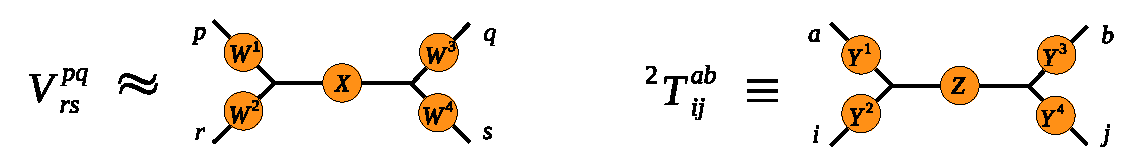
\includegraphics[width=0.95\textwidth]{figures/rccsd_thc_def}}.
\label{fig:rccsd_thc_def}
\end{equation}
%
As diagrams show, two electron interaction is decomposed in Mulliken order, as 
well as two body excitation amplitudes. To study the properties of THC-RCCSD 
we calculated energies of a set of small to medium size weakly correlated 
molecules.

In our setup the decomposition of the electron interaction tensor was 
calculated with a two step method, as described in 
Ref.~\cite{schutski2017tensor} First, partial singular value decomposition of 
the integrals in AO basis was calculated. We retained $r_{V}$ singular values 
and vectors. For larger systems, listed in Tab.~\ref{Tab:Energies}, RI 
decomposed two electron integrals were used in place of singular 
vectors. Next, a CP decomposition of rank $r_{V}$ of the resulting 
left and right singular vectors (arranged as three index tensors of size $N 
\times N \times r_{V}$) was calculated with ALS. The iterative least squares 
procedure was stopped when the ratio of the objective function $f$ to the 
square of the Frobenius norm of the original tensor dropped below $10^{-14}$, or 
a limit of 1000 iterations was reached.

In the subsequent coupled cluster calculations we chose the rank of THC 
decomposition of ${}^2T$ amplitudes ($r_{T}$) to be equal to the rank 
used in approximating integrals, e.g. $r_{T} = r_{V}$. 
The CC iterations were stopped either after the energy was converged to within 
$10^{-9}$ Hartree or a limit of 250 iterations 
was reached. All calculations used the cc-pVDZ basis from EMSL
database,\cite{schuchardt2007basis} and the corresponding cc-pVDZ-RI
was used in the RI approximation. The threshold for pseudoinverses was set to 
$10^{-10}$.

\section{Accuracy of THC for two electron integral approximation}
The accuracy of the THC decomposition of the two-electron integrals governs the
accuracy of the energy in subsequent calculations. Thus, it is important to 
check the dependence of the error in the decomposition of
two-electron integrals on THC rank. Figure~\ref{fig:thc_err_mo_3systems} plots 
this error in a double logarithmic scale for three small molecules. Once again, 
we note that the decomposition is computationally useful if the rank 
$r_\mathrm{V}$ is close to the number of basis functions $N$.  As the figure 
shows, the error in the two-electron integrals decreases exponentially with
respect to THC rank. We found that this trend holds for every system
tested. Further, there is no significant difference whether the two-electron 
integrals are decomposed in the atomic orbital or molecular orbital basis, as 
is demonstrated in Figure~\ref{fig:thc_err_ao_vs_mo}.

%
\begin{figure}[tb]
%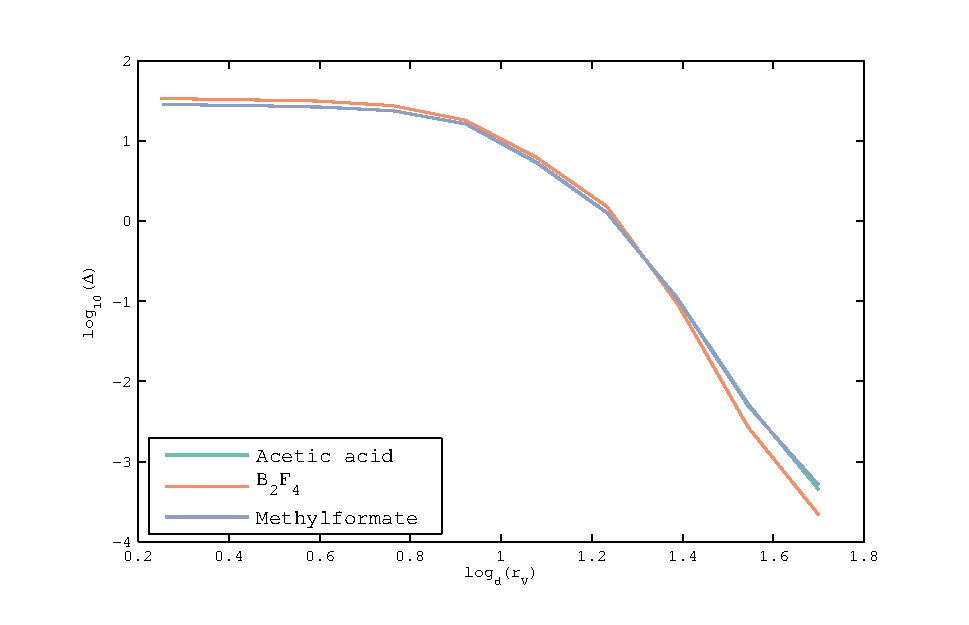
\includegraphics[width=\columnwidth]{figures/thc_err_mo_3systems}
\caption{Frobenius norm of error in decomposed two electron integrals.
\label{fig:thc_err_mo_3systems}}
\end{figure}
%
\begin{figure}[tb]
%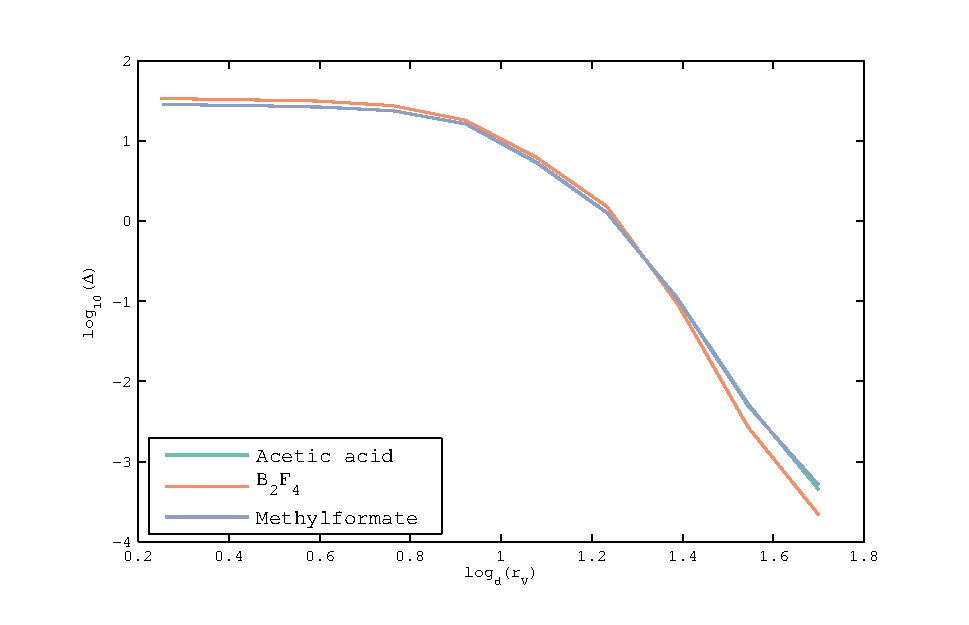
\includegraphics[width=\columnwidth]{figures/thc_err_mo_3systems}
\caption{Frobenius norm of error in decomposed two electron integrals of Acetic 
Acid in atomic and molecular orbital bases.
\label{fig:thc_err_ao_vs_mo}}
\end{figure}
%

To see how these errors of the THC approximation of two-electron 
integrals influence the accuracy of subsequent energies, we checked 
the error in the second-order M{\o}ller-Plesset (MP2) correlation
energy, as shown in Fig.~\ref{fig:mp2_err_ao_full}.  The combination
of MP2 and THC was first proposed by Hohenstein \emph{et
al}.\cite{hohenstein_thc2} and scales as $O(N^4)$.  The way these authors were 
calculating THC decomposition, however, was quite different from ours.
As we found, the error in the MP2 correlation energy follows the trend seen in 
the decomposition of the two-electron integrals (see 
Fig.~\ref{fig:mp2_err_ao_full}). Results within $0.1~mH$
of the exact MP2 correlation energy are already achieved with
$r_\mathrm{V} \sim N^{1.2} - N^{1.4}$.
We expect that the THC would work even better for larger and more extended 
systems as the two-electron integrals become sparser and a lower rank 
decomposition would correspondingly become more accurate.
%
\begin{figure}[tb]
%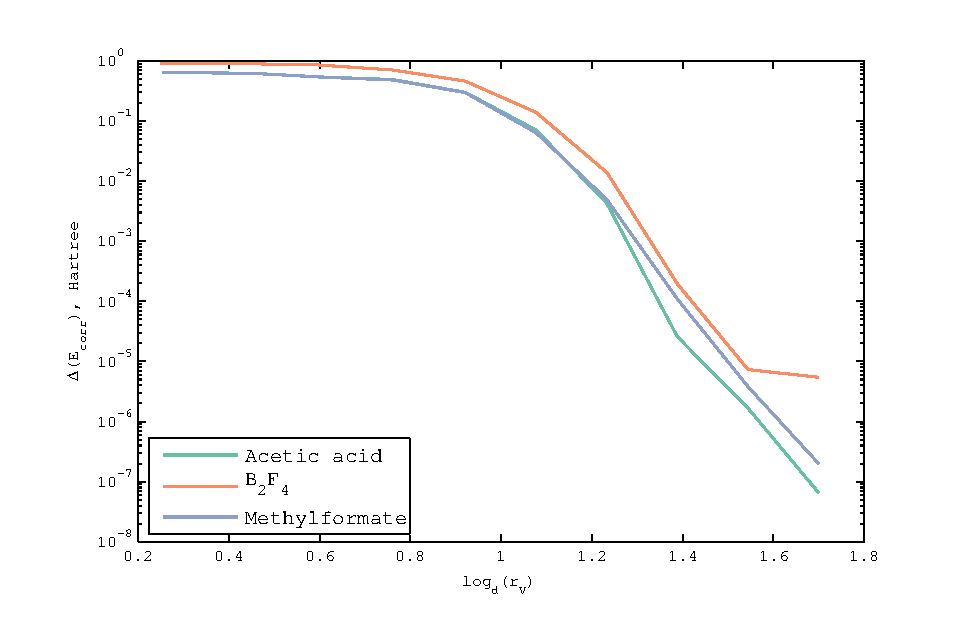
\includegraphics[width=\columnwidth]{figures/mp2_err_ao_full}
\caption{Absolute error in the MP2 correlation energy.
\label{fig:mp2_err_ao_full}}
\end{figure}
%
\section{Accuracy of THC-RCCSD}
We are up to demonstrate the accuracy the THC-decomposed RCCSD
method. Note that we set the rank in THC of amplitudes to equal the rank 
used in the decomposition of two electron integrals. The error in the RCCSD 
correlation energy has a non-monotonic dependence on THC rank, but follows the 
same basic trends as seen in Fig.~\ref{fig:thc_err_mo_3systems} and
Fig.~\ref{fig:mp2_err_ao_full}. Similarly to the case of MP2, errors on 
the order of $0.1~mH$ are achieved with $r_\mathrm{T} = r_\mathrm{V} \sim 
N^{1.2} - N^{1.4}$.
%
\begin{figure}[tb]
%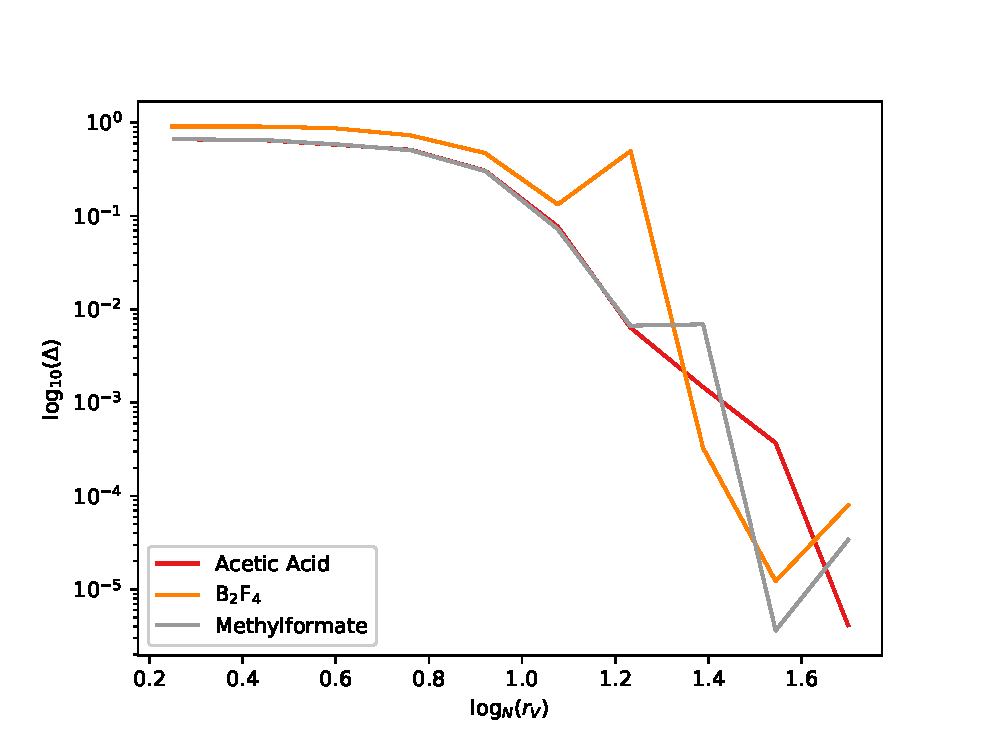
\includegraphics[width=\columnwidth]{figures/cc_err_ao_full}
\caption{Absolute error in the RCCSD correlation energy.
\label{fig:cc_err_ao_full}}
\end{figure}
%
It is interesting to estimate what part of the error in energy can be
attributed to the approximation of the Hamiltonian only. For this reason we 
calculated the correlation energy with converged THC-RCCSD amplitudes but exact
two-electron integrals.  As Fig.~\ref{fig:cc_err_ao_full_amps_only}
shows, using the exact two-electron integrals substantially decreases the error 
in energy, which later motivated us to look for better ways of decomposing the 
two electron integrals. The non-monotonic behavior of the error (as compared to 
MP2) can be attributed to the nonlinear nature of the coupled cluster 
equations, which can be quite sensitive to changes in the parameters of the 
Hamiltonian.
%
\begin{figure}[tb]
%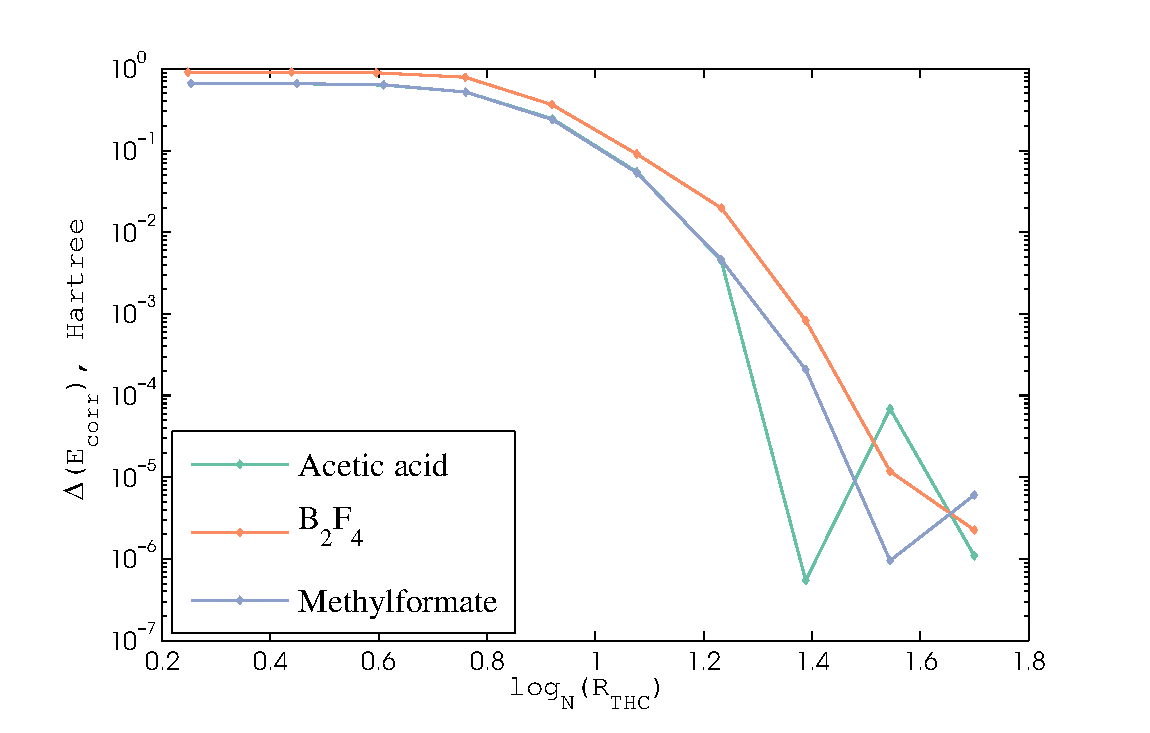
\includegraphics[width=\columnwidth]{figures/cc_err_ao_full_amps_only}
\caption{Absolute error in the RCCSD correlation energy with exact two
electron integrals.
\label{fig:cc_err_ao_full_amps_only}}
\end{figure}
%
\section{{More numerical examples of THC-RCCSD}
\label{sec:more_examples_thc}}
Having checked the properties of THC-RCCSD on few small systems, we 
tested the method on a larger set of small and medium-sized molecules introduced 
in previous work on THC.\cite{hohenstein_thc3} Technical details of the 
calculations, including molecular geometries and reference energies, are 
provided in the supplementary materials of Ref.~\cite{schutski2017tensor}. We 
chose the ranks of the THC decomposition of the amplitudes and integrals to be 
on the same scale as the number of auxiliary basis functions $N_\mathrm{RI}$ 
used in the standard RI approximation. In Table~\ref{Tab:Energies} we list 
energies, differences with respect to regular Coupled Cluster, the number of CC 
iterations and norm of final residuals. We used RI for all these calculations 
in the first step of THC decomposition of the two electron integrals. 
%
\begin{center}
\begin{table}[h]
\caption{CCSD correlation energies ($E_c$), errors in
correlation energies ($\Delta E_c$), number of THC-RCCSD iterations 
($n_{iter}$) 
and the norm of doubles residuals ($|{}^2R_{ij}^{ab}|$) for several small 
molecules.
\label{Tab:Energies}}
\begin{tabular}{lccccccc}
& & \multicolumn{2}{c}{$\Delta E_c (mH)$} & \multicolumn{2}{c}{$n_{iter}$} & 
\multicolumn{2}{c}{$|{}^2R_{ij}^{ab}|$}\\
\cline{3-4} \cline{5-6} \cline{7-8} System & $E_c (mH)$ & $N_\mathrm{RI}$ &
$1.5 \, N_\mathrm{RI}$ & $N_\mathrm{RI}$ &
$1.5 \, N_\mathrm{RI}$ & $N_\mathrm{RI}$ &
$1.5 \, N_\mathrm{RI}$\\
\hline
Acetic acid & -666.510 & -0.579 & -0.453 & 50 & 31 & 0.041 & 0.033 \\
Aniline & -997.193 & -1.177 & -0.471 & 111 & 64 & 0.051 & 0.032 \\
Diboron tetrafluoride & -909.944 & -0.702 & -0.716 & 15 & 17 & 0.053 & 0.034\\
Benzene & -823.101 & -0.985 & -0.450 & 111 & 62 & 0.048 & 0.030\\
Butadiene & -581.340 & -0.710 & -0.274 & 41 & 42 & 0.041 & 0.025\\
Cyclobutane & -621.099 & -0.895 & -0.290 & 77 & 50 & 0.039 & 0.028\\
Dimethylsulfoxide & -661.870 & 0.195 & -0.624 & 287 & 39 & 0.056 & 0.025\\
Furan & -736.463 & -0.865 & -0.454 & 73 & 50 & 0.046 & 0.033\\
Isobutane & -652.505 & -0.876 & -0.263 & 78 & 49 & 0.035 & 0.025\\
Methylformate & -666.805 & -0.586 & -0.455 & 62 & 35 & 0.042 & 0.032\\
Methylnitrite & -708.990 & -0.476 & -0.492 & 68 & 47 & 0.047 & 0.033\\
Phenol & -1005.727 & -0.887 & -0.514 & 120 & 59 & 0.051 & 0.032\\
Pyridine & -842.453 & -1.045 & -0.475 & 104 & 61 & 0.047 & 0.032\\
Pyrrole & -727.051 & -0.855 & -0.407 & 84 & 52 & 0.045 & 0.032\\
Thiophene & -695.593 & -1.013 & -0.657 & 97 & 52 & 0.039 & 0.032\\
Toluene & -980.030 & -1.270 & -0.461 & & & &\\
\hline
MUE\footnote{mean unsigned error} & & 0.820 & 0.466 & & & &\\
Max\footnote{maximum unsigned error} & & 1.270 & 0.716 & & & &\\
RMS\footnote{root-mean-square error} & & 0.861 & 0.482 & & & &\\
\end{tabular}
\end{table}

\end{center}
%
Let us highlight an important finding in 
Table~\ref{Tab:Energies}. As THC-RCCSD is an approximation to regular CC 
equations, the full residuals may not be zero, because the number of CC 
equations is usually much larger than the number of parameters of THC-RCCSD. 
An interesting observation is that despite the norm of 
doubles residuals is not negligible in THC-RCCSD, the error in energy 
is quite low. This contrasts with conventional CC, where the 
difference of energy during iterations with the converged value  
is of the same order as the norm of the residual. This fact is explored in 
more detail in the next chapter. 

Overall, THC-RCCSD provides a viable approximation to conventional RCCSD and 
should be orders of magnitude faster per iteration, especially for large basis 
sizes $N$. It should be noted, however, that most of the time in our 
calculations was spent on the decomposition of the Hamiltonian rather
than on the solution of approximated CC equations. 
One way to overcome this problem is to use quadrature based methods for 
building THC, such as the ones described in Refs.~\cite{hohenstein_thc1} 
and~\cite{parrish2013discrete}. These methods may be much
faster than iterative approaches we employed, at the expense of 
using about 3x larger ranks to reach the same 
accuracy.\cite{parrish2013discrete} Another way is to avoid THC decomposition 
of two electron integrals altogether, as is described in the next 
chapter.

\section{Convergence of THC-RCCSD}
Finally, let us discuss the convergence of the THC-RCCSD. In this 
work we used a simple iterative algorithm to solve THC-RCCSD equations, 
and stoped iterations when a specified difference in energy between subsequent 
steps was reached. The convergence of the resulting algorithm significantly 
depends on the rank of the THC approximation. 
Figure~\ref{fig:cc_thc_convergence} shows the number of iterations the algoritm 
had to take to reach $\theta = 1\cdot 10^{6} H$ difference in energy.
%
\begin{figure}[tb]
%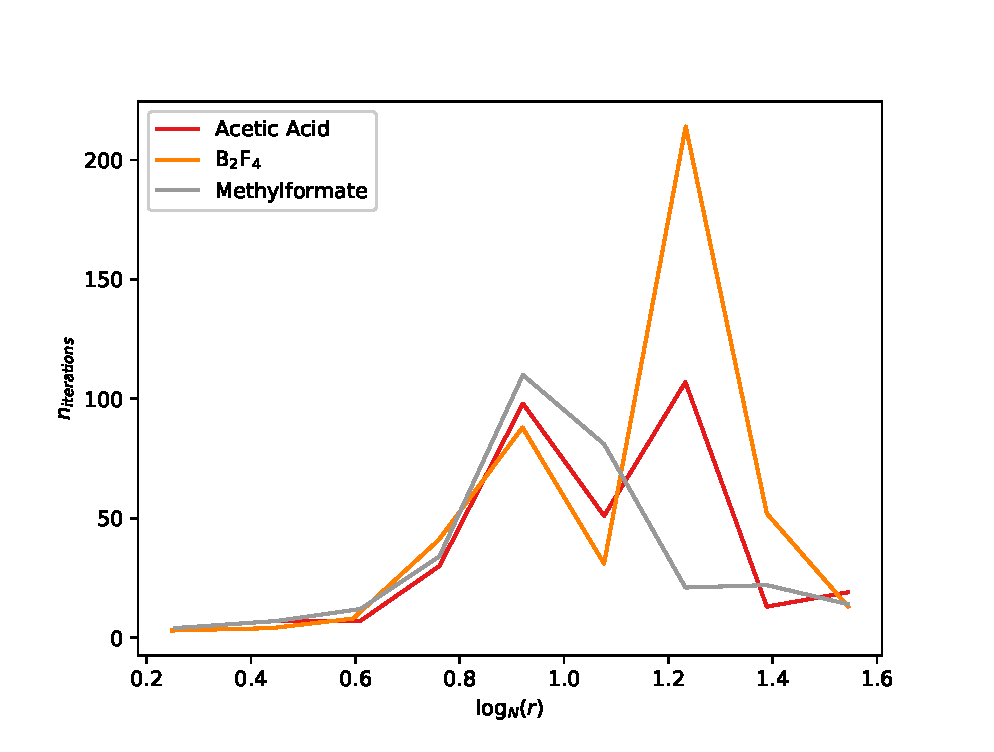
\includegraphics[width=\columnwidth]{figures/niter_vs_logr}
\caption{Number of iterations of THC-RCCSD to reach $1 \cdot 10^{-6} H$ 
difference in energy}
\label{fig:cc_thc_convergence}
\end{figure}
%
For small as well as larger THC ranks the convergence of THC-RCCSD is 
comparable or better than regular RCCSD (if simple iterations were used). In 
the intermediate regime, however, the algorithm may need
a large number of iterations to converge. We note that the convergence in this 
regime significantly depended on the choice of initial parameters and several 
random trials needed to find good ones. We provide the following tentative 
explanation to the observed behavior. As 
THC-RCCSD in our formulation is a sum of two iterative algorithms, merely, an 
ALS step and a CC iteration, there is a competition between 
updates each of these parts is generating. In case of small ranks the update 
should be mostly determined by ALS, as ${}^{2}T$ amplitudes are poorly 
approximated with any set of parameters $Y$. In 
contrast, with larger ranks mostly CC equations govern the update, because 
${}^2T$ is well approximated at each step. We admit, however, that the means to 
control convergence of our hybrid algorithms 
need a further study. All later numerical experiments were done in a regime 
where THC-RCCSD performs similarly to regular RCCSD, e. g. where THC ranks are 
relatively large. 


\appendix

%\include{append-a}
%\appendix
%\addcontentsline{toc} {chapter}{\numberline {}Appendix A}  
%\include{append-a}
%\include{append-b}
%\addcontentsline{toc} {chapter}{\numberline {}Bibliography}{}
%\include{biblio}

\bibliographystyle{ieeetr}
\bibliography{references}
\end{document}
